\chapter{Chapter 4. Grad-Shafranov reconstruction and automated identification algorithm} \label{ch:ch4} % of magnetic structures

\section{The Grad-Shafranov equation}
%\input{Chapters/Introduction/GS_equation}
The Grad-Shafranov (GS) equation describes the force balance between the Lorentz force and the gradient of the thermal pressure \citep{Sonnerup:1996, Hau:1999}, as given below,
\eql{eq:GS}{\delsq A = \npdv{2}{A}{x} + \npdv{2}{A}{y} = -\mu_0 \dv{P_t}{A} = - \mu_0\dv{}{A}\p{p + \frac{B_z^2}{2\mu_0}}.}

\subsection{Derivation of the original GS equation}
Starting with the magnetic field as a function of the magnetic vector potential and balancing the gradient of the pressure with the Lorentz force,
\eql{eq:B}{\Bvec = \delcross\Avec = \del\Avec\cross\zhat + B_z\zhat}
\eql{eq:gradp}{\grad p = \jvec\cross\Bvec = j_z\zhat\cross\Bvec_\perp + \jvec_\perp\cross B_z\zhat}

\noindent Using Ampere's law to determine the components of the current density $\jvec$,
\eql{eq:Amperes}{\begin{split}
    \delcross\Bvec &= \mu_0\jvec \\
    \delcross\p{\delcross\Avec} & = \mu_0\jvec \\
    \delcross\pp{\grad\Avec\cross\zhat + B_z\zhat} &= \mu_0\pp{j_z\zhat + \jvec_\perp} \\
\end{split}}
The $\zhat$ and perpendicular components of the current density are then found by,
\eql{eq:jz}{\begin{split}
    \mu_0 j_z\zhat &= \delcross\p{\grad\Avec\cross\zhat} \\
    &= \p{\deldot\zhat}\grad\Avec - \p{\deldot\del\Avec}\zhat \\
   j_z\zhat &= -\frac{1}{\mu_0}\delsq\Avec\zhat \\
\end{split}}
\eql{eq:jperp}{\begin{split}
    \mu_0\jvec_\perp &= \delcross B_z\zhat \\
    \jvec_\perp &= \frac{1}{\mu_0}\grad B_z\cross\zhat \\
\end{split}}

\noindent Simplifying the $\zhat$ and perpendicular terms of the pressure gradient (\ref{eq:gradp}),
\eql{eq:jzBperp}{\begin{split}
    j_z\zhat \cross\Bvec_\perp &= -\frac{1}{\mu_0}\delsq\Avec\zhat\cross\p{\grad\Avec\cross\zhat} \\
    &= -\frac{1}{\mu_0}\pp{\p{\delsq\Avec\zhat\cdot\zhat}\del\Avec - \p{\delsq\Avec\zhat\cdot\grad\Avec}\zhat} \\
    &= -\frac{1}{\mu_0}\p{\delsq\Avec} \grad\Avec \\
\end{split}}
\eql{eq:jperpBz}{\begin{split}
    \jvec_\perp\cross B_z\zhat &= \p{\frac{1}{\mu_0}\grad B_z\cross\zhat}\cross B_z\zhat \\
    &= \frac{1}{\mu_0}\pp{\p{\zhat\cdot\del}B_z\zhat - \p{B_z\zhat\cdot B_z\zhat}\del} \\
    &= -\frac{1}{\mu_0}B_z\grad B_z
\end{split}}

\noindent and substituting them into the respective right hand side of (\ref{eq:gradp}), we arrive at the form for the Grad-Shafranov equation (\ref{eq:GS}):
\eq{\begin{split}
    \grad p &= -\frac{1}{\mu_0}\p{\delsq\Avec}\grad\Avec - \frac{1}{\mu_0}B_z\grad B_z \\
    \p{\delsq\Avec}\grad\Avec &= -\mu_0\p{\grad p+ \frac{1}{\mu_0}B_z\grad B_z} \\
    \p{\delsq\Avec}\grad\Avec &= -\mu_0 \p{\dv{p}{A}\grad\Avec + \frac{1}{\mu_0}B_z\dv{B_z}{A}\grad\Avec} \\
    \delsq\Avec &= -\mu_0\p{\dv{p}{A} + \frac{1}{\mu_0}\dv{B_z}{A}} \\
\end{split}}

\eql{eq:gradp2}{\delsq\Avec = -\mu_0\dv{}{A}\p{p + \frac{B_z^2}{2\mu_0}}}

%https://agupubs.onlinelibrary.wiley.com/doi/10.1029/2006JA011717
\subsection{Derivation of the extended GS equation}
The implementation by \cite{Chen:2021} utilizes the extended GS method, which still seeks to find the double-folding pattern between two $P_t'$ versus $A'$ curves, but with $A'=(1-\alpha)A$ and $P_t'=\p{1-\alpha}p + \p{1-\alpha}^2\frac{B_z^2}{2\mu_0} + \alpha\p{1-\alpha}\frac{B^2}{2\mu_0}$.  The factor $\alpha$ is a proportionality constant, which for a field-aligned flow is the average Alfv\'en Mach number squared, $\alpha=\langle M_A\rangle^2 \approx const$ in a frame of reference moving with the structure governed by the GS equation. The extended GS equation \citep{Teh:2018, Sonnerup:2006} is:
\begin{equation}
    \nabla^2 A' = -\mu_0\frac{\mathrm{d}}{\mathrm{d}A'}\left[\left(1-\alpha\right)p + \left(1-\alpha\right)^2\frac{B_z^2}{2\mu_0} + \alpha\left(1-\alpha\right)\frac{B^2}{2\mu_0} \right]
    \label{eq:GSextended}
\end{equation}
which simplifies to the original GS equation (\ref{eq:GS}) when $\alpha\equiv 0$. The extended GS method allows us to identify structures with significant remaining plasma flow aligned with the local magnetic field in a proper frame of reference \citep{Chen:2022}.

\section{Automated GS-based detection of SFRs}
In both the original and the GS-type equations, the transverse pressure $P_t$, and its equivalent $P_t'$, are single variable functions of the magnetic flux function $A$ ($A'$ for the GS-type with $\alpha\equiv const$). With this feature, one can recover the 2D cross-section of a flux rope structure from the 1D spacecraft data by solving the initial value problem based on the GS equation, i.e., by carrying out the GS reconstruction procedures \citep{Hau:1999, HuSonnerup:2002, Hu:2017}. The GS-based techniques in this study consist of the GS-type reconstruction and the extended GS-based automated detection. Considering the complicated environment from the solar wind to the magnetosheath, we adopt the GS-type reconstruction in this study for selected events only.

A cross section of a cylindrical flux rope structure is fully characterized by the 2D scalar flux function $A(x, y)$, and the field-line invariants $\p{B_z,J_z,p, P_t}$ vary among the nested cylindrical flux surfaces while remaining constant on each distinct surface with a distinct $A$ value \citep{Hu:2018}. As a spacecraft passes through the cross section of a magnetic flux rope with closed transverse field lines, it crosses the same set of magnetic field lines twice, the second time being in reverse order as the first half of the crossing. Therefore, the measured magnetic flux function $A$ associated with the field lines traversed by the spacecraft is double-folded, meaning there is a turning point at which an extremum in $A$ is reached. These features, especially the double-folding pattern, are the basis for the GS reconstruction-based identification algorithm \citep{Hu:2018}. Figure \ref{fig:GSreconstruction_Hu2017} shows diagram of a reconstruction of a magnetic cloud event and the associated flux rope structure. The cross section from the reconstruction algorithm can be seen as well as its relation to the magnetic field lines of the flux rope structure. A more detailed description of the implementation \citep{Hu:2018}, including a flowchart of the flux rope detection algorithm, can be found in Appendix \ref{appendix:gs-flowchart}, and online\footnote{\url{fluxrope.info/flowchart.html}}.

\begin{figure}
    \centering
    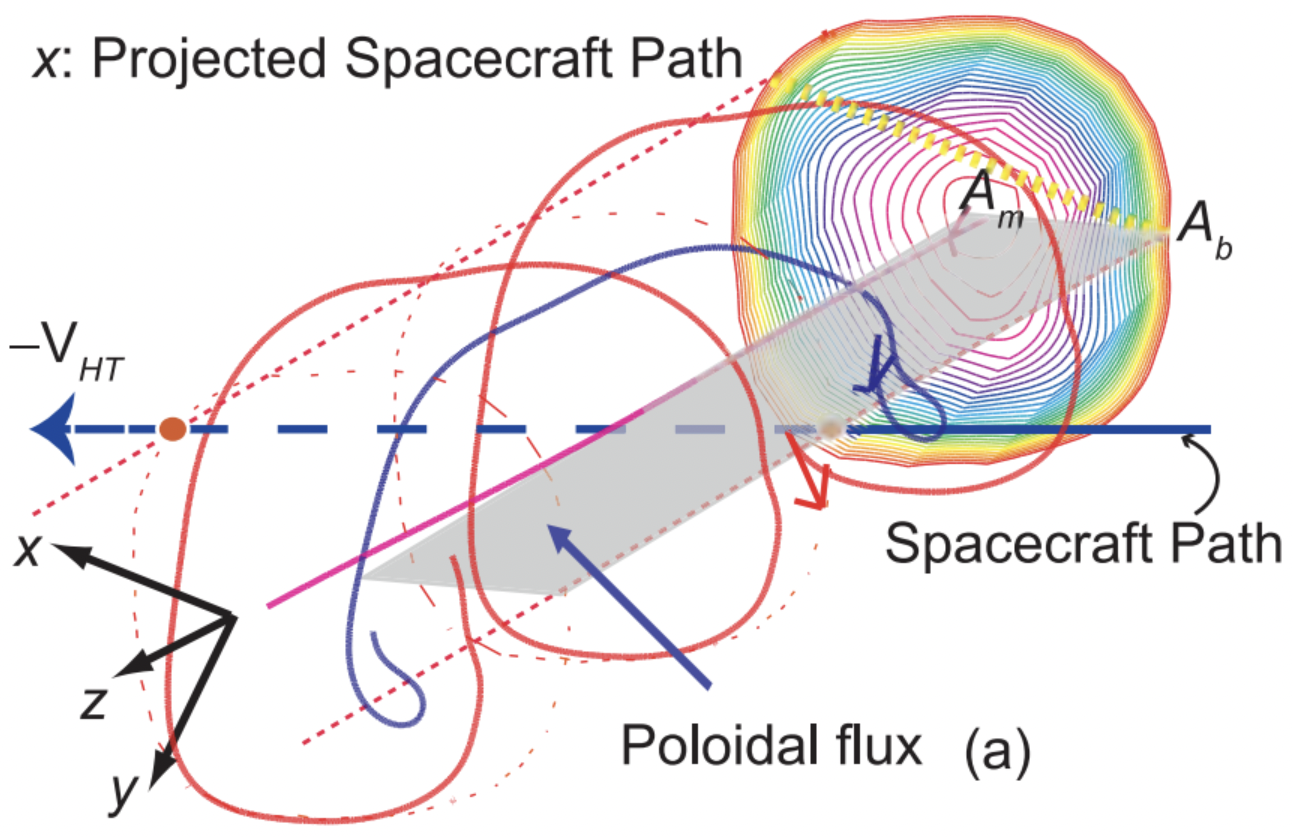
\includegraphics[width=0.75\textwidth]{Figures/Hu2017_5a.png}
    \caption[2D cross section view of a flux rope structure reconstruction] {View of a flux rope structure reconstruction for a magnetic cloud event \citep{Hu:2015} as a spacecraft passes through it. The 2D cross section and selected associated magnetic field lines (red and blue twisted lines) along the flux rope axis ($z$-axis). $A_m$ and $A_b$ mark the magnetic flux function $A$ at the center and boundary, respectively, of the reconstruction. The poloidal flux can also be obtained through the reconstruction algorithm.} %$\Phi_p = |A_m-A_b|\cdot L_{eff}$ along the effective length of the $z$-axis (shaded portion)
    \label{fig:GSreconstruction_Hu2017}
\end{figure}

% Determination of the cylindrical z-axes
The GS-based algorithm starts by moving a window continually through an entire data segment with variable window sizes in turn, ranging from the minimum duration of approximately 10 data points with cadence $\Delta t$, i.e. 10$\Delta t$, to the maximum duration of 343 data points to cover a wide range of SFR duration, while taking into account limited computing resources. The maximum duration corresponds to approximately 17 minutes for the THEMIS data, and 25 minutes for the MMS data. The \textit{in situ} magnetic field and plasma data from a specified window of time are first transformed into the co-moving frame, notably the de Hoffmann-Teller frame \citep{deHoffman-Teller:1950}. Through a trial-and-error process, the optimal orientation of the $z$-axis is determined. A trial $z$-axis is represented by the azimuthal and polar angles, $\phi$ and $\theta$, in the GSE coordinate system. The azimuthal angle $\phi$ is the longitude of the SFR $z$-axis, which measures the angle between the GSE $X$-direction and the projection of the $z$-axis onto the $XY$-plane. The polar angle $\theta$ is the angle between the SFR $z$-axis and the $Z$-direction. To do so, we select trial values for $\phi$ and $\theta$, and calculate the transverse pressure $P_t'$ along the spacecraft path, as shown in Equation (\ref{eq:GSextended}). The plot of $P_t'$ versus $A'$ may have a turning point where $P_t'$ along the spacecraft path splits into two parts, with an extreme $A'$ value near this turning point, typically for an SFR structure. This is where the magnetic field $B_y$ component changes sign because of the field line geometry of a helical structure. Figure \ref{fig:Pt-vs-A} represents such a $P_t'$ versus $A'$ plot, with two distinct portions joining near a turning point with a minimum $A'$ value. We evaluate the quality of the folding (or overlapping) of the two parts of $P_t'$ versus $A'$ by two metrics, $R_{diff}$ (the point-wise difference residue between the two parts) and $R_{fit}$ (a residue of the fitting function $P_t'(A')$ as illustrated by the solid black curve). These metrics are used to check how well the two parts fold onto each other, provided that such a turning point exists. The threshold conditions, $R_{diff}\lesssim 0.2$ and $R_{fit}\lesssim 0.2$ for these metrics, are selected empirically to guarantee good double-folding quality \citep{Hu:2018}. We are able to find the optimal orientation of the $z$-axis of the SFR by going through iterations of $\phi$ and $\theta$ until the minimum residue values are found. Once the minimum residues satisfying the threshold conditions are found, the corresponding optimal $z$-axis orientation and event interval are recorded as an SFR candidate.

\begin{figure}
    \centering
    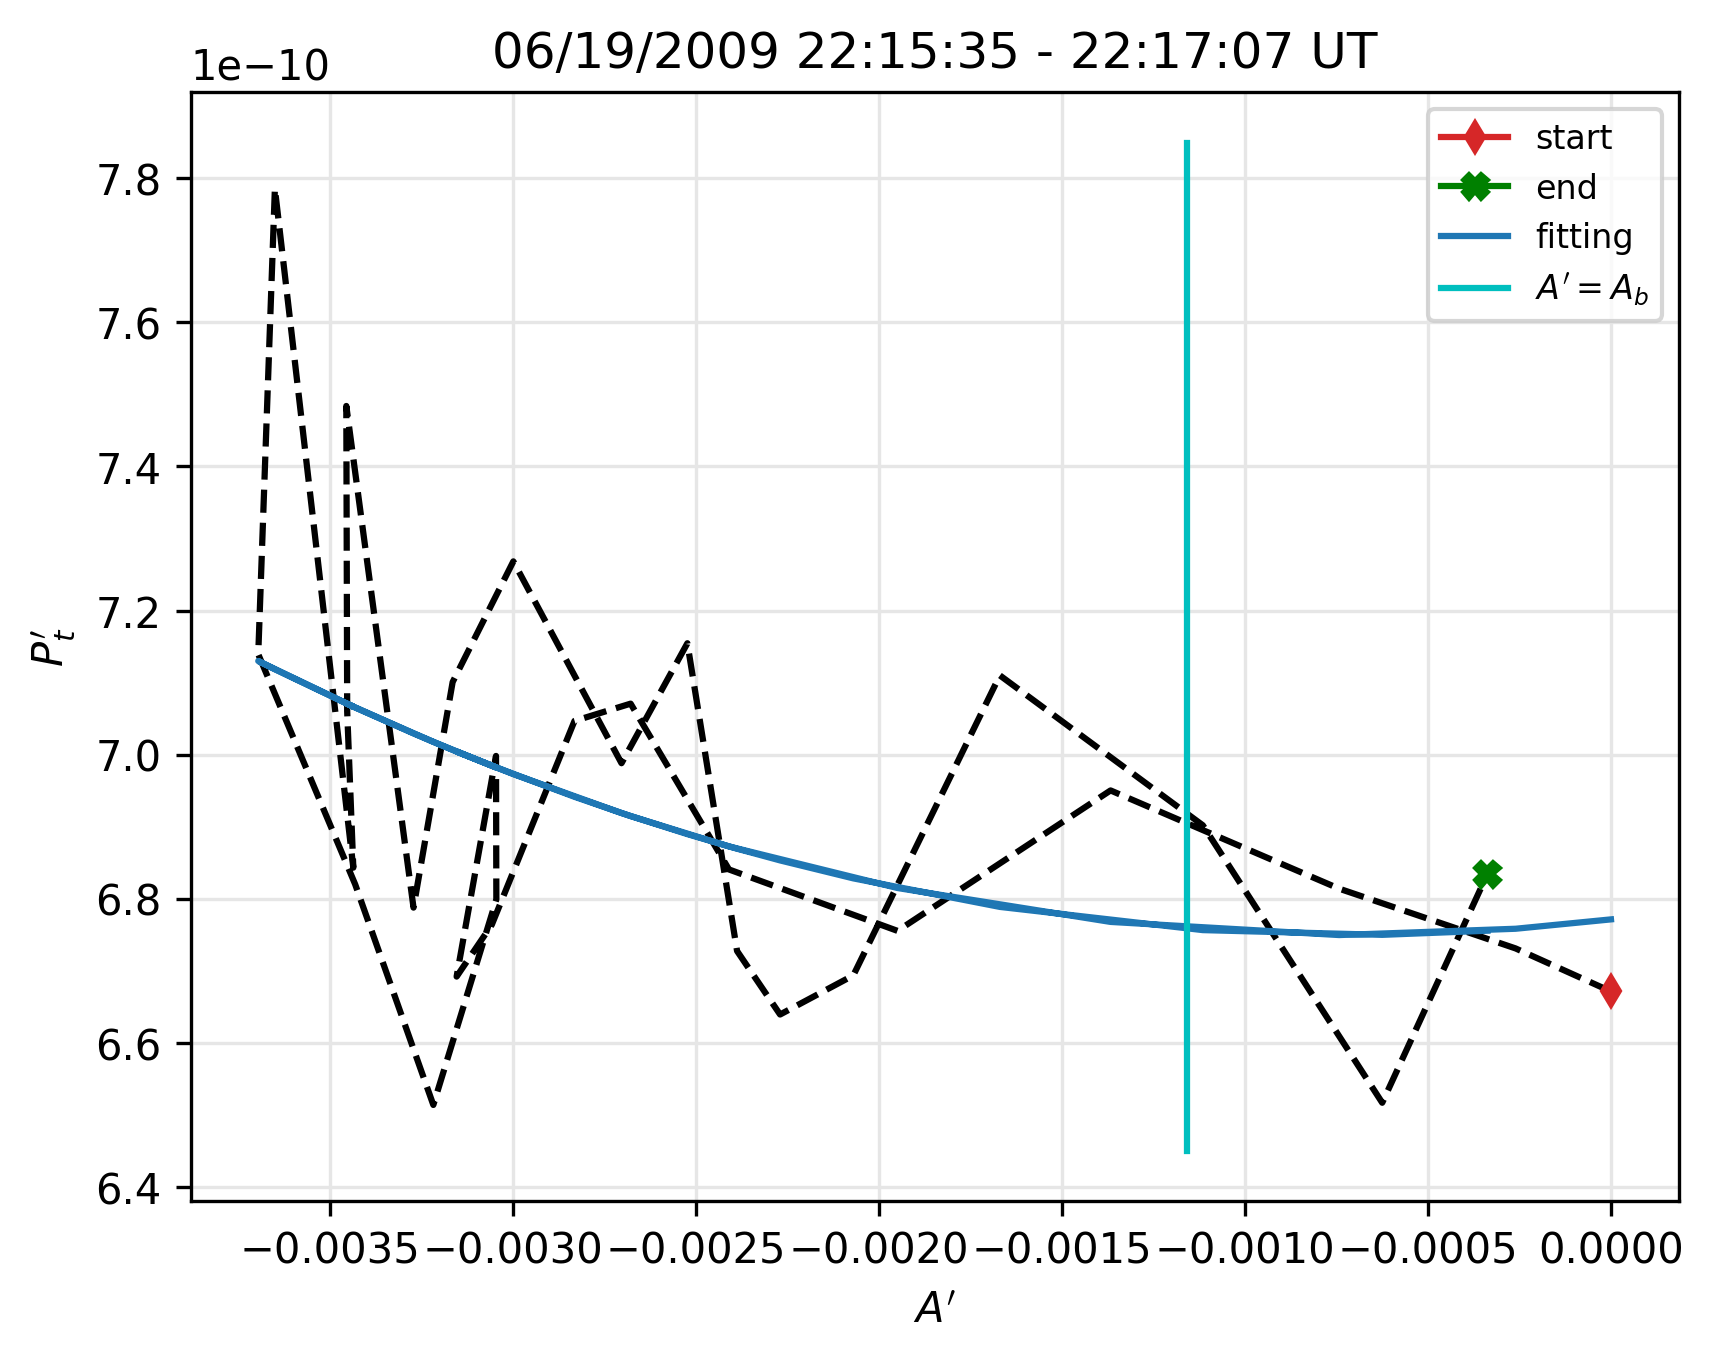
\includegraphics[width=\textwidth]{Figures/Reconstructions/PtvsA_Ab_20090619_20090621.png}
    \caption[Double folding pattern of $P_t'$ versus $A'$ for 22:15:35-22:17:05 UT on 19 June 2009]{$P_t'(A')$ versus $A'$ plot for an SFR from 22:15:35-22:17:05 on 19 June 2009 observed by THM-C. The red and green markers indicate the starting and ending points of the SFR interval, the darker blue line indicates the fitted $P_t'(A')$ versus $A'$ function, and the lighter blue line indicates the turning point where $A'=A_b$.}
    \label{fig:Pt-vs-A-Ab}
\end{figure}

\begin{figure}
    \centering
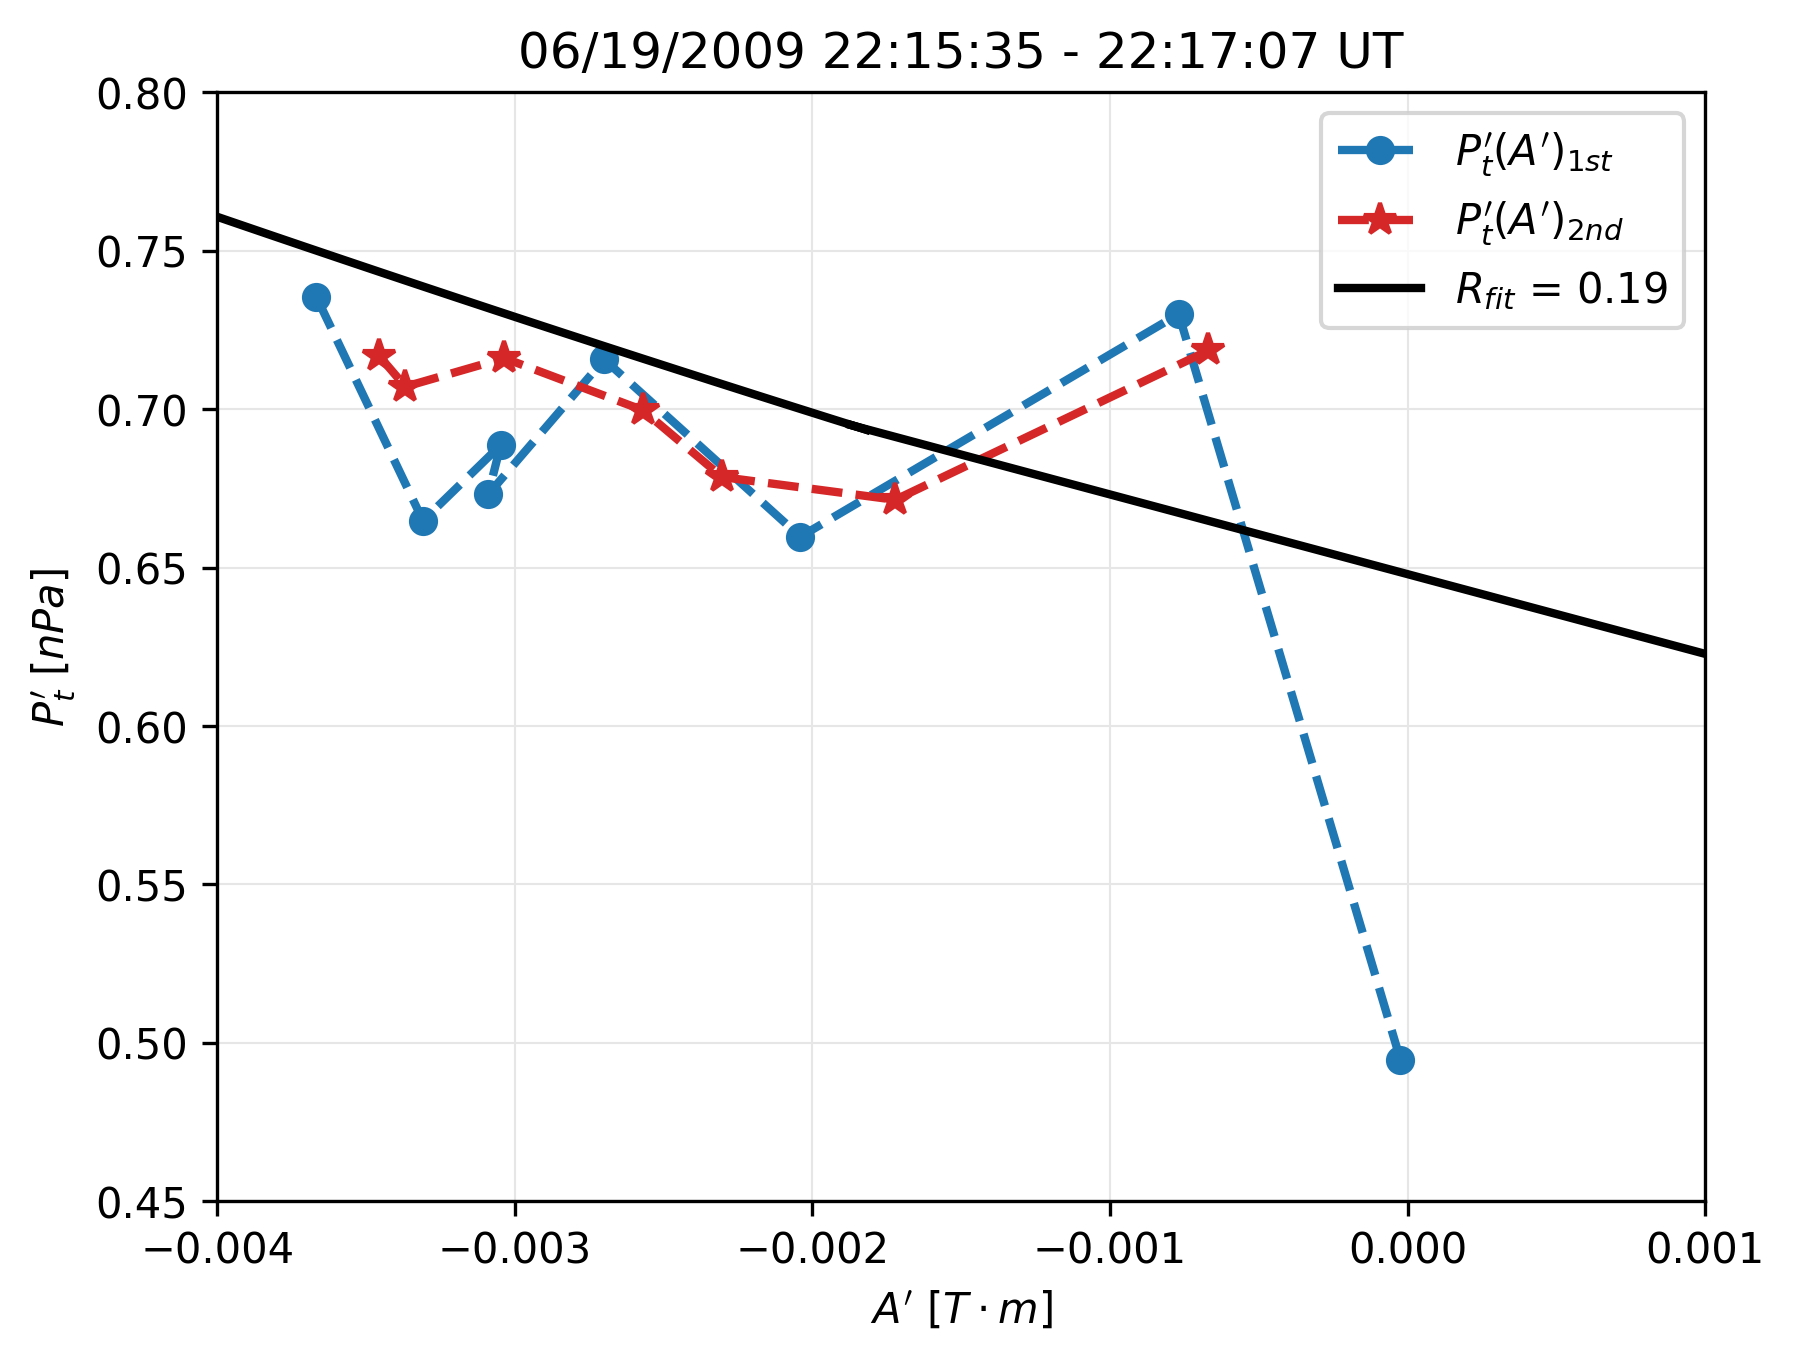
\includegraphics[width=\textwidth]{Figures/Reconstructions/PtvsA_20090619_20090621.png}
    \caption[$P_t'$ versus $A'$ plot for 22:15:35-22:17:05 UT on 19 June 2009]{The $P_t'$ versus $A'$ plot for an SFR interval from 22:15:35-22:17:05 UT on 19 June 2009 observed by THM-C. The data points are marked by the symbols, and are connected by the blue dashed line and the red dashed line, separated by the turning point at the minimum of $A'$ in this case. The two lines correspond to the first and second parts of the $P_t'(A')$ curve as denoted by the legend. The solid black curve represents a functional fitting to the data points with fitting residue $R_{fit}$.}
    \label{fig:Pt-vs-A}
\end{figure}

% The data are then used to calculate the transverse pressure $P_t'(A')$ as a function of the scalar flux function, $A'$. If the $P_t'$ versus $A'$ is double folded through a flux rope interval, then two metrics, $R_{diff}$ (the point-wise difference between the two folds) and $R_{fit}$ (a fitting residue of $P_t'(A')$), are used to check the double-folding quality and the shape of $P_t'(A')$. The threshold values for these metrics are selected empirically to guarantee good flux rope quality \citep{Hu:2018}, and if the thresholds are met, the event is recorded as an event candidate. If the thresholds are not met, the $z$-axis will go through its next iteration until the thresholds are met.

After the initial detection of SFR candidates, the list of initial candidates is refined. The records are further classified based on the Wal\'en test slope $w$. Records with $|w|\leq0.3$ are quasi-static SFRs and thus saved directly. Records with $|w|>0.3$, except for when the correlation coefficient $r$ between the aforementioned two velocities ($\mathbf{V_{sw}} - \mathbf{V_{HT}}$ and $\mathbf{V_A}$) is $|r|\geq 0.8$ and $\langle M_A\rangle \leq 0.9$, are removed. These conditions ensure that the remaining plasma flow is aligned with the local magnetic field, and also to avoid a singularity in Equation (\ref{eq:GSextended}) at $\alpha=1$. Events with $\alpha>1$ are rare, but they are also removed, so that the events remaining are sub-Alfv\'enic. We also remove events from the initial candidate list if the candidates have a turning point within $5\Delta t$ (turn time) of the turning point of another candidate with a smaller $R_{diff}$, as these could be the same overlapping structures. Table \ref{tab:thresholds} lays out the threshold conditions as utilized in the post-processing of the GS-based detection event list \cite{Chen:2020, Chen:2021, Chen:2022}. The duration of the search windows does not exceed 343$\Delta t$ ($\sim 25.733$ minutes for MMS and $\sim 24.553$ minutes for THEMIS) due to computational time constraints. The detection algorithm was performed for some time periods with search window size up to 388 points in duration; however, the search yielded very few (generally less than 3) additional event counts after the post-processing steps. This was due to the step of making sure there is no overlap between SFR candidates, which prioritizes smaller duration candidates. Therefore, with the search algorithm taking a significant amount of time to run for longer search windows and yielding very few results, it was decided to stop the search at the maximum window size of $343\Delta t$. The PyGS software used to reconstruct the 2D cross-section of the events can be found at \url{https://github.com/PyGSDR/PyGS}.
\begin{table}[h!]
\centering
\caption[Threshold conditions for GS algorithm]{Table of threshold conditions for GS reconstruction-based algorithm. $R_{diff}$ and $R_{fit}$ are residues which ensure good double-folding quality in the $P_t'(A')$ vs. $A'$ curve..} %Events meeting the following criteria are kept.} %Duration is $10*dt\sim 343*dt$ where $dt\sim 3$ seconds.
\begin{tabular}{ccccccc}
\toprule
    Duration  & $R_{diff}$ & $R_{fit}$ & Turn time & Wal\'en test slope & $|r|$ & $\langle M_A\rangle$ \\ 
    \hline
    %$\sim$ 30-1029 & $<0.2$ & $<0.2$ & 5$dt$ & $\leq 1$ &  &  \\
    10$\Delta t$-342$\Delta t$ & $<0.2$ & $<0.2$ & 5$\Delta t$ & $|k|\leq 0.3$ & & \\
    10$\Delta t$-342$\Delta t$ & $<0.2$ & $<0.2$ & 5$\Delta t$ & $|k|> 0.3$ & $\geq 0.8$ & $\leq 0.9$ \\
\bottomrule %30-1029 (s)
\end{tabular}
\label{tab:thresholds}
\end{table}

%Solar wind
%k <= 0.3:  1752
%k > 0.3; r>|0.8|, <M_A> <0.9:  107

% Magnetosheath
%k <= 0.3:  2310
%k > 0.3; r>|0.8|, <M_A> <0.9:  70


\begin{figure}
    \centering
    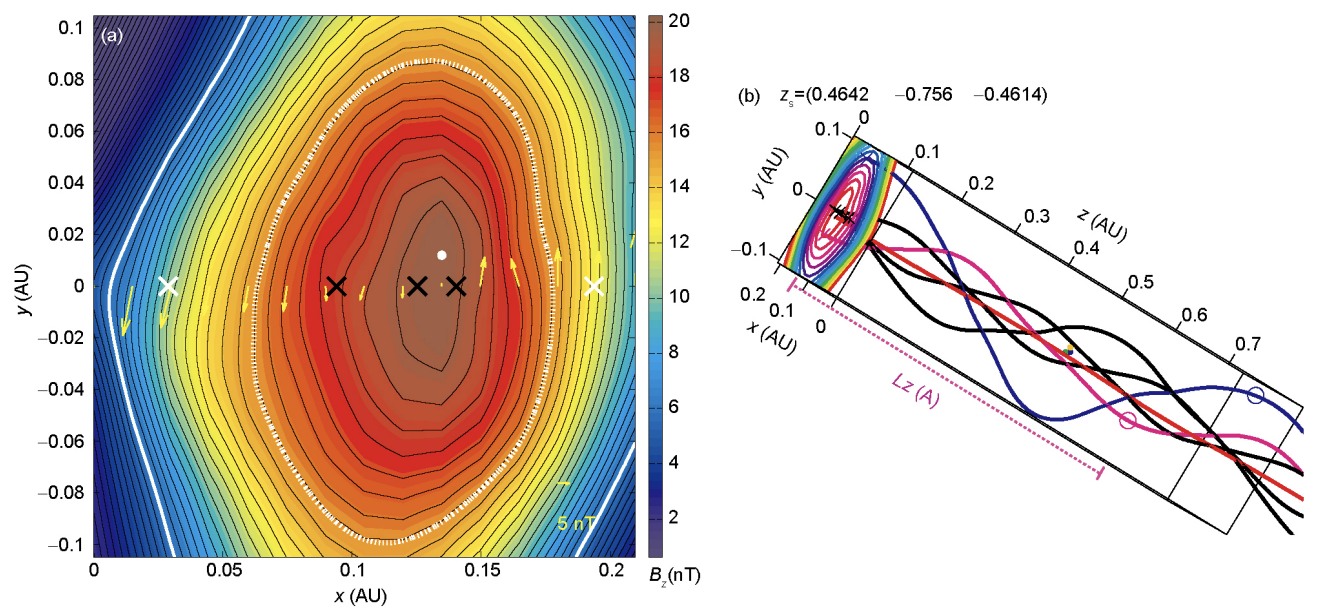
\includegraphics[width=\textwidth]{Figures/Reconstructions/Hu2015_GSreconstruction.png}
    \caption[GS 2D reconstruction of a magnetic cloud]{Reconstruction of a magnetic cloud \citep{Hu:2015}: a) 2D cross section of $A(x,y)$ for a reconstructed magnetic cloud event. The black lines indicate the transverse magnetic field lines, and the color bar indicates the axial field lines $B_z$. The yellow arrows denote the transverse field lines ($B_t$) along the path of the spacecraft ($y=0$). The white contour indicates the area of the reconstruction done from spacecraft data ($A=A_b$), while the area outside the white contour is reconstructed from extrapolation. b) 3D view of a flux rope structure for the magnetic cloud event, showing the 2D cross section (A') and selected associated twisted magnetic field lines along the flux rope axis (denoted at the top). The black field lines  rooted at the foot points where the electron onsets were observed. The pink and blue circles denote the locations where the associated field lines complete a full turn around the z-axis.}
    \label{fig:GSreconstruction_Hu2015}
\end{figure}

%Such an extended version searches FRs including those with significant field-aligned flows as they also meet the broad definition of magnetic flux ropes, \textit{i.e}., having twisted field lines around the central axis \citep{Chen:2021}. Therefore, the Alfv\'enicity of these dynamic structures is not negligible, which will be characterized by the $M_A$ and the Wal\'en test slope.

\section{Wal\'en test and Alfv\'enicity}
The Wal\'en test slope $w$, the slope of the linear regression between $\mathbf{V_{sw}} - \mathbf{V_{HT}}$ and $\mathbf{V_A}$, is then used to further distinguish Alfv\'enic structures

%generalized test is most simply formulated as a vector difference equation relating changes in the electron velocity vector and changes of the magnetic field vector, with a prescribed scalar constant of proportionality.

\section{Analysis results}
\begin{figure}
    \centering
    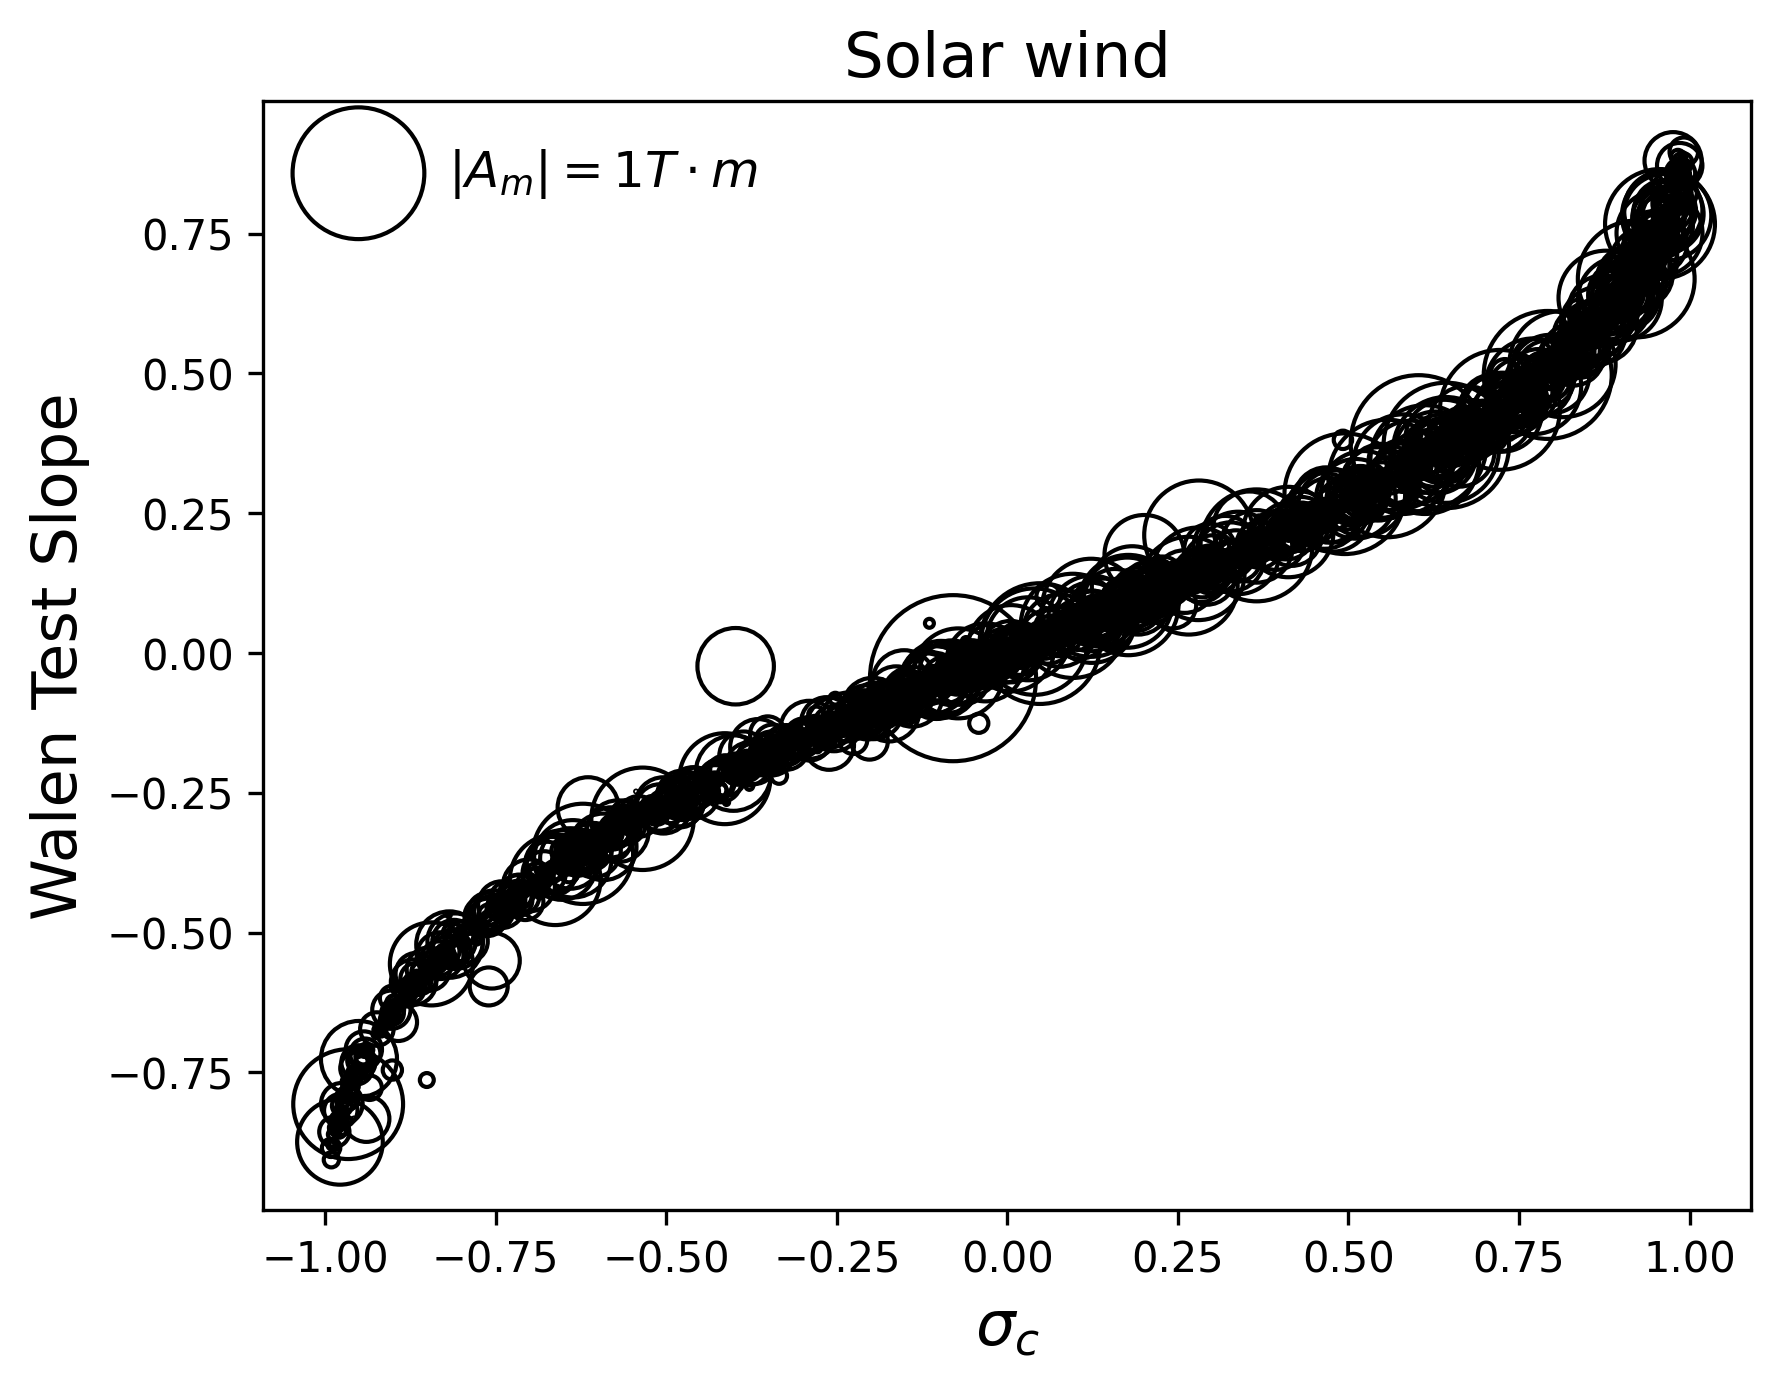
\includegraphics[width=0.45\linewidth]{Figures/GS analysis/walenTest_vs_crosshelicity_solarwind.png}
    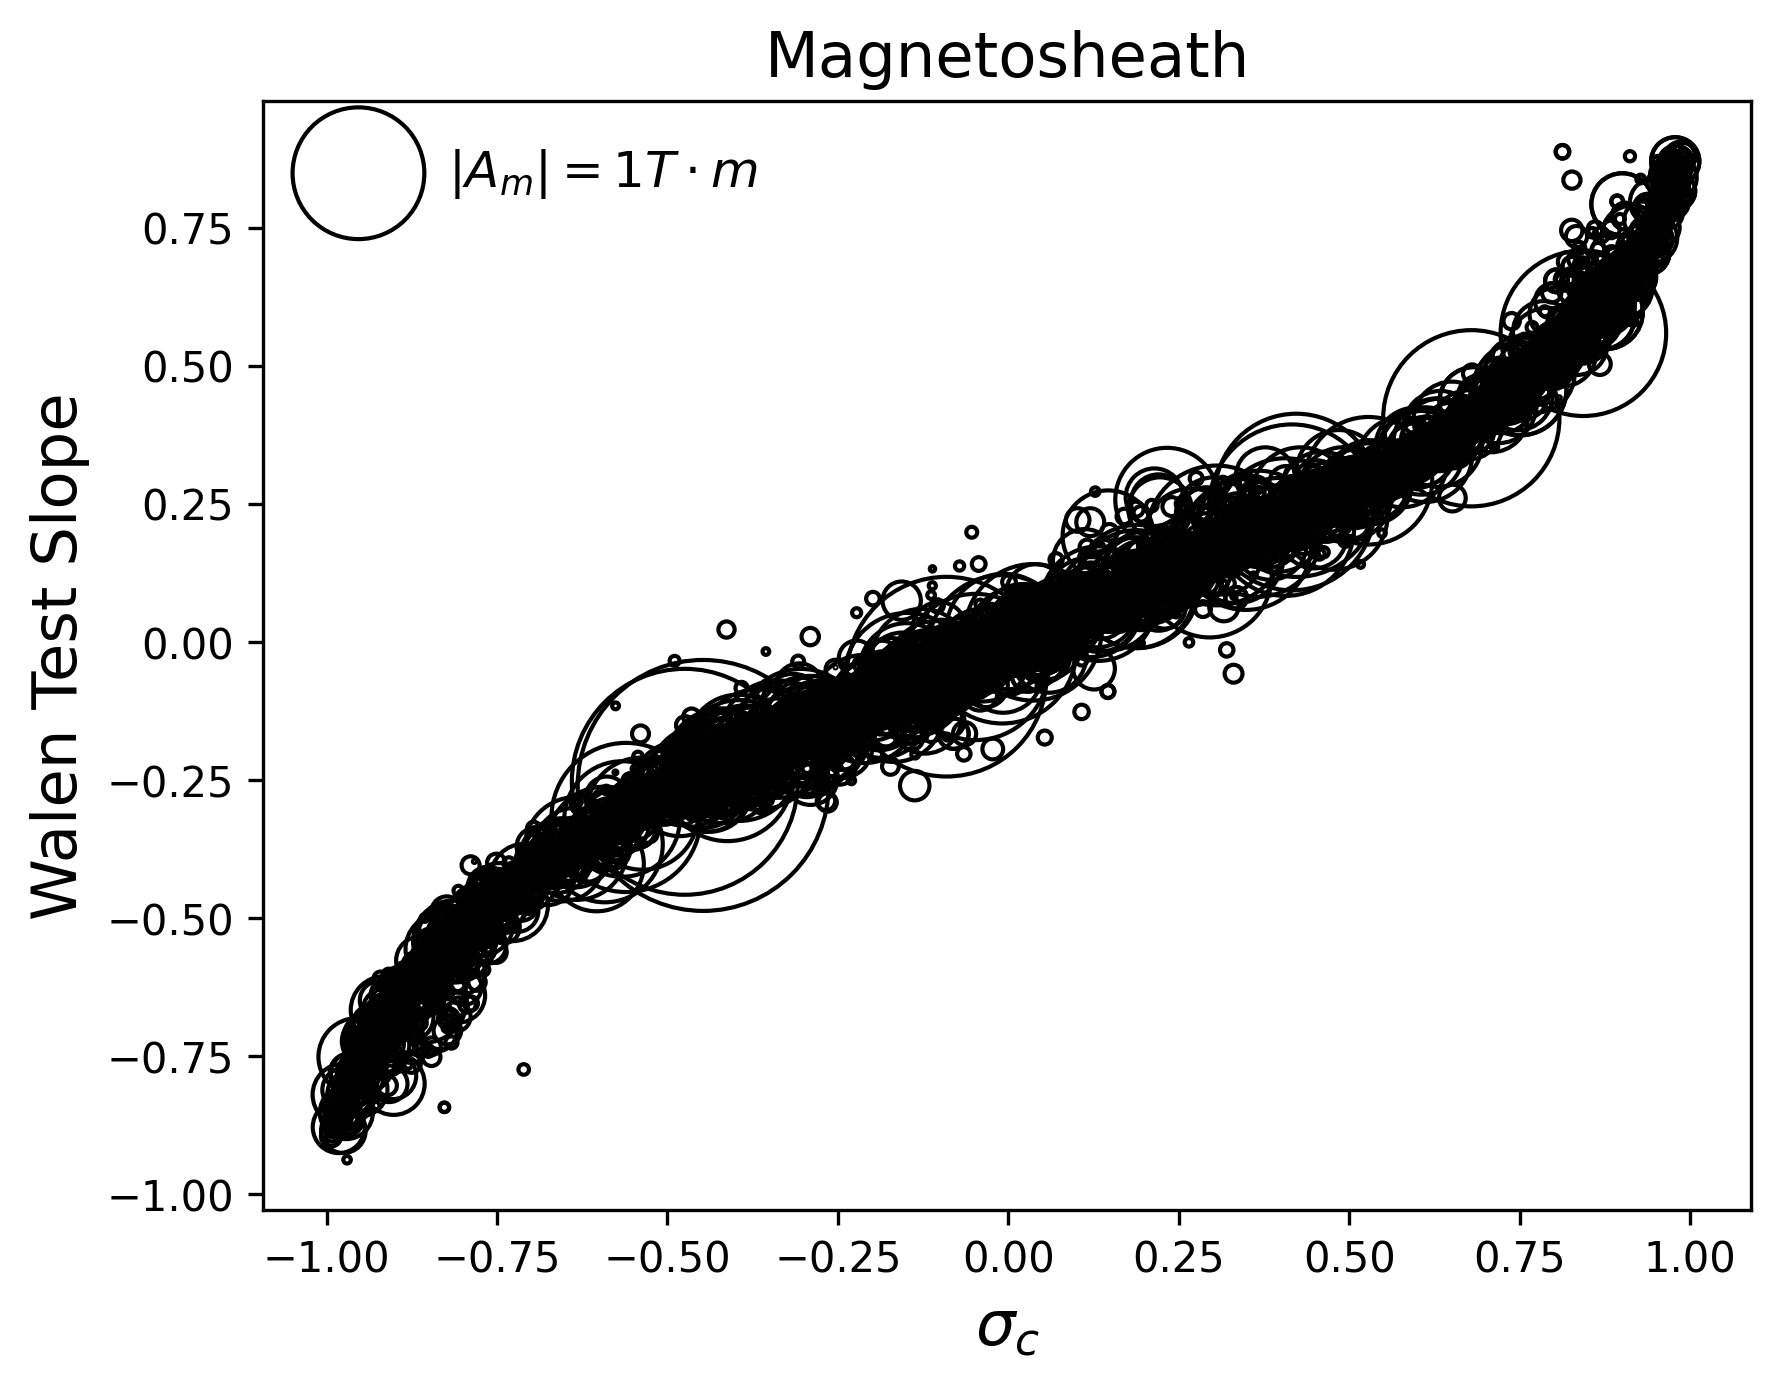
\includegraphics[width=0.45\linewidth]{Figures/GS analysis/walenTest_vs_crosshelicity_magnetosheath.png}
    \caption[Wal\'en test slope vs. reduced cross helicity]{Caption}
    \label{fig:walen-crosshelicity}
\end{figure}


\begin{figure}
    \centering
    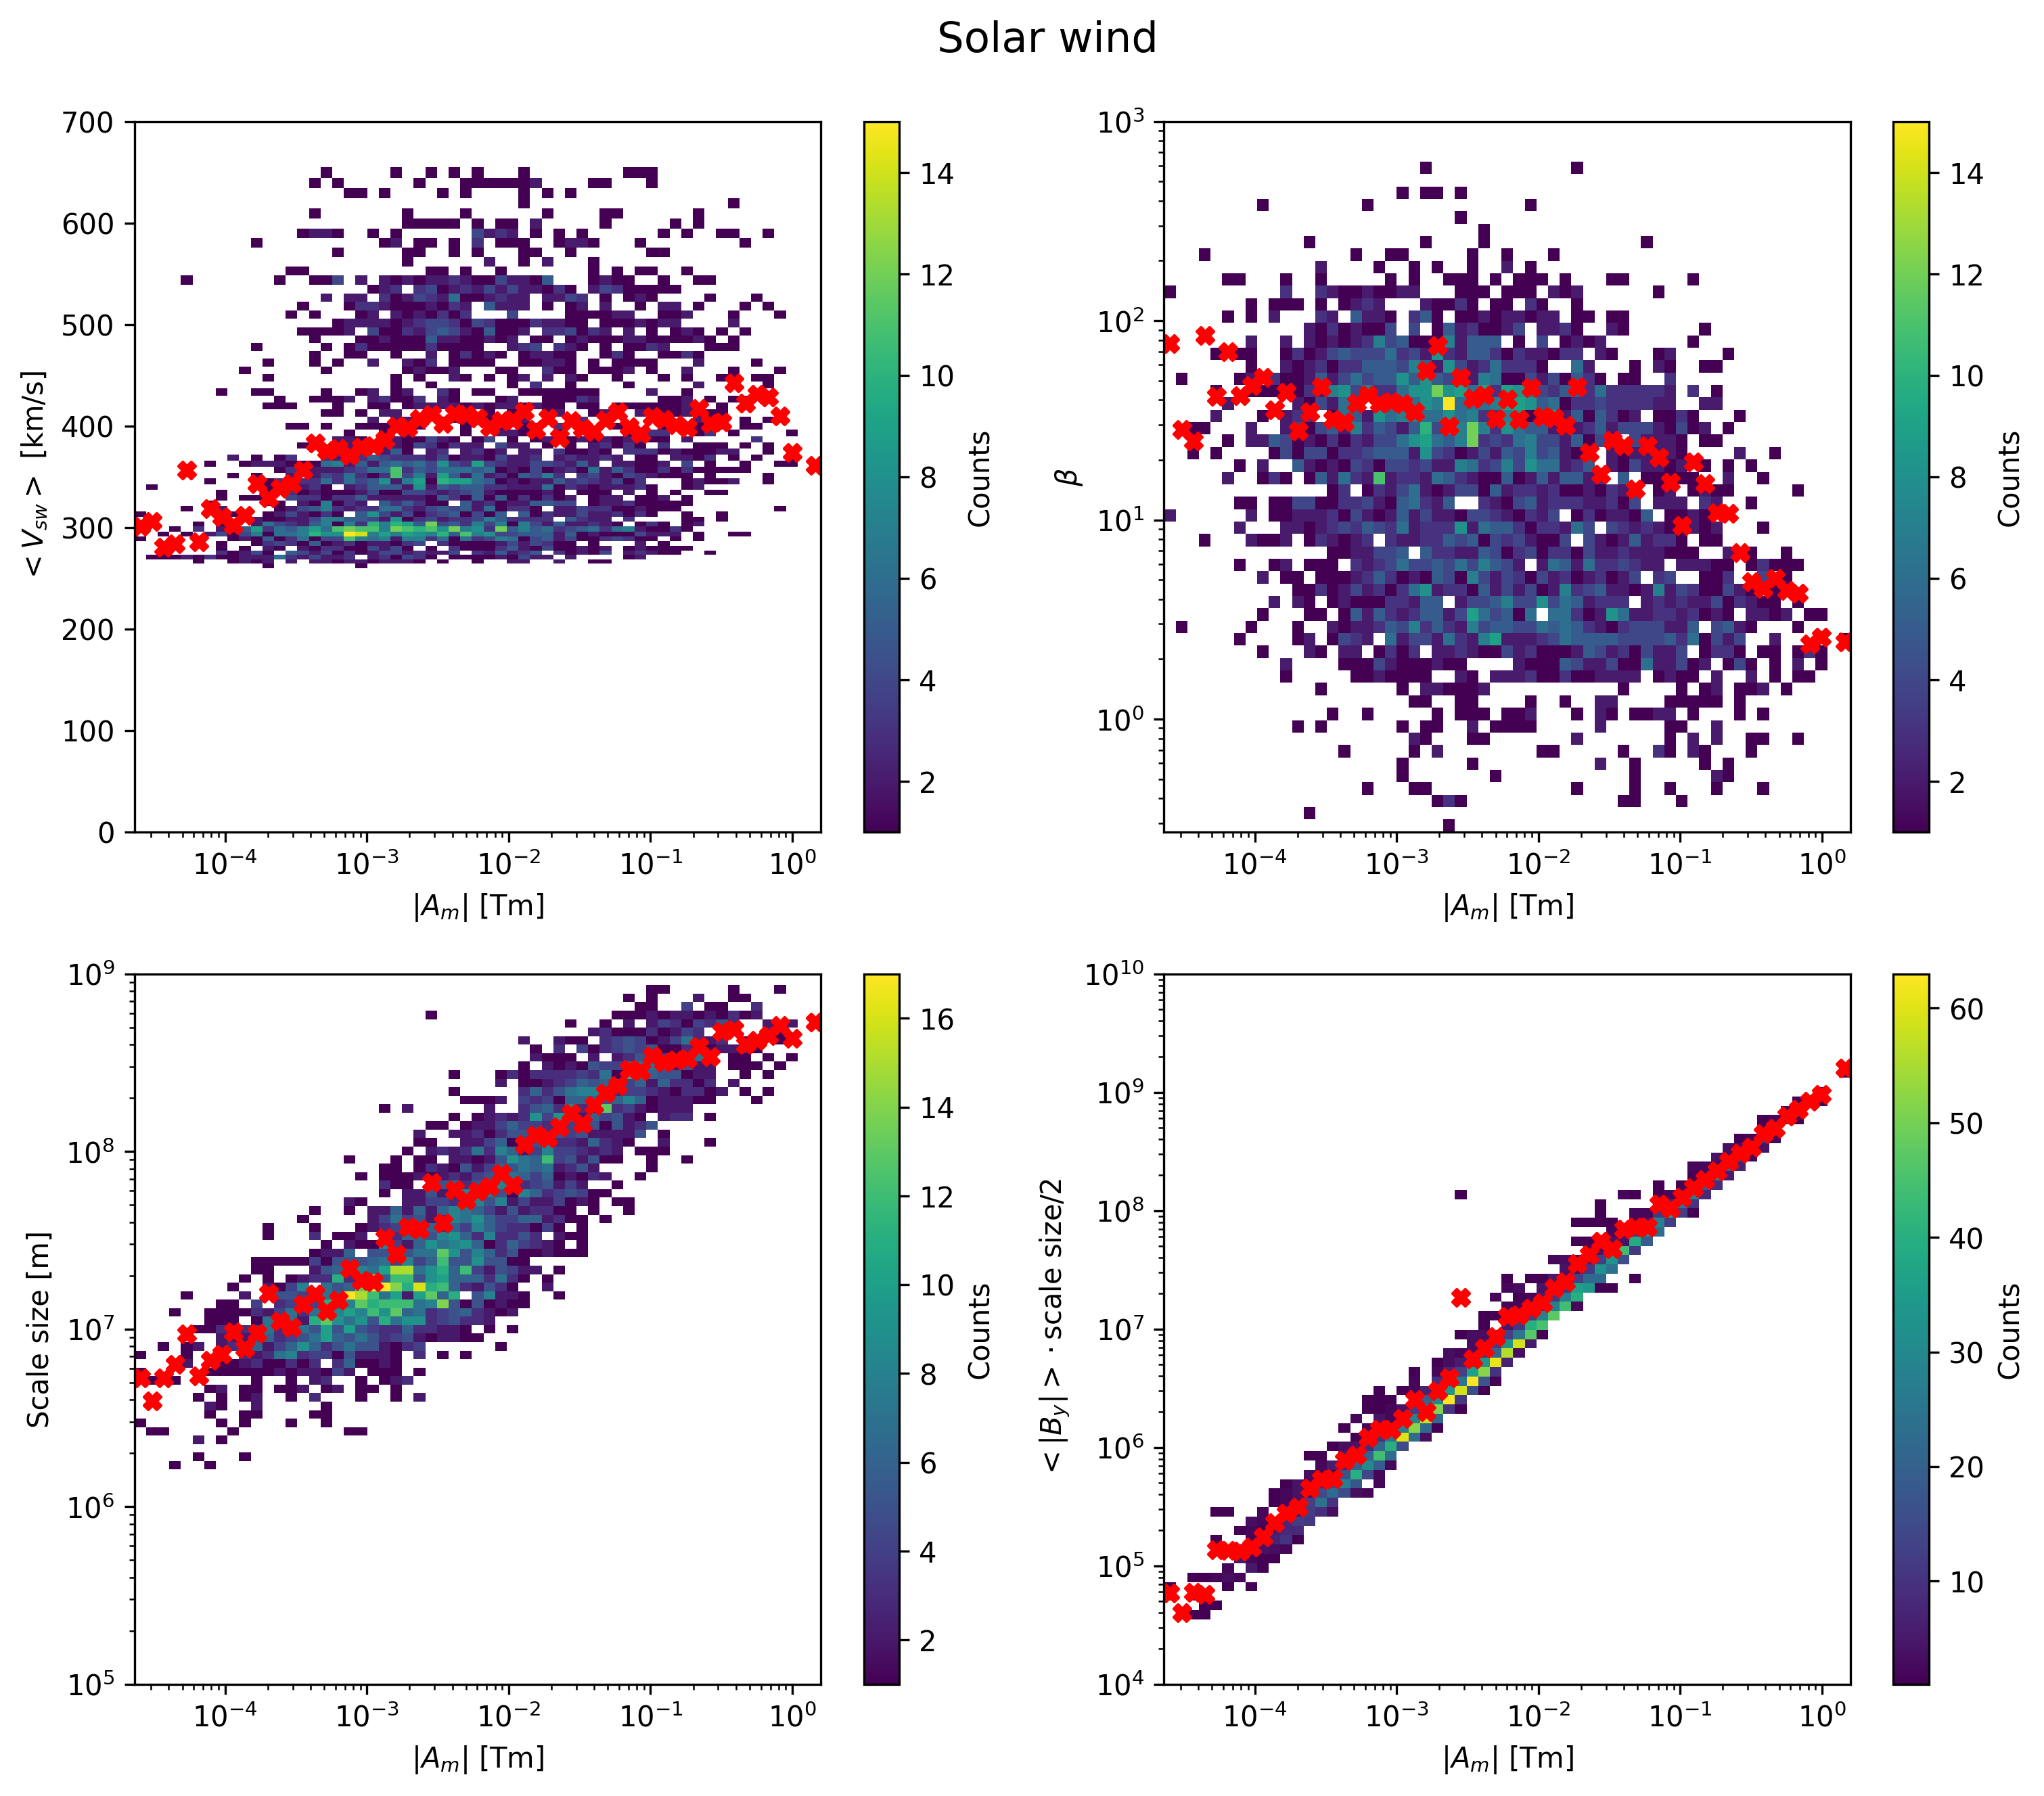
\includegraphics[width=0.45\linewidth]{Figures/GS analysis/heatmap_solarwind.png}
    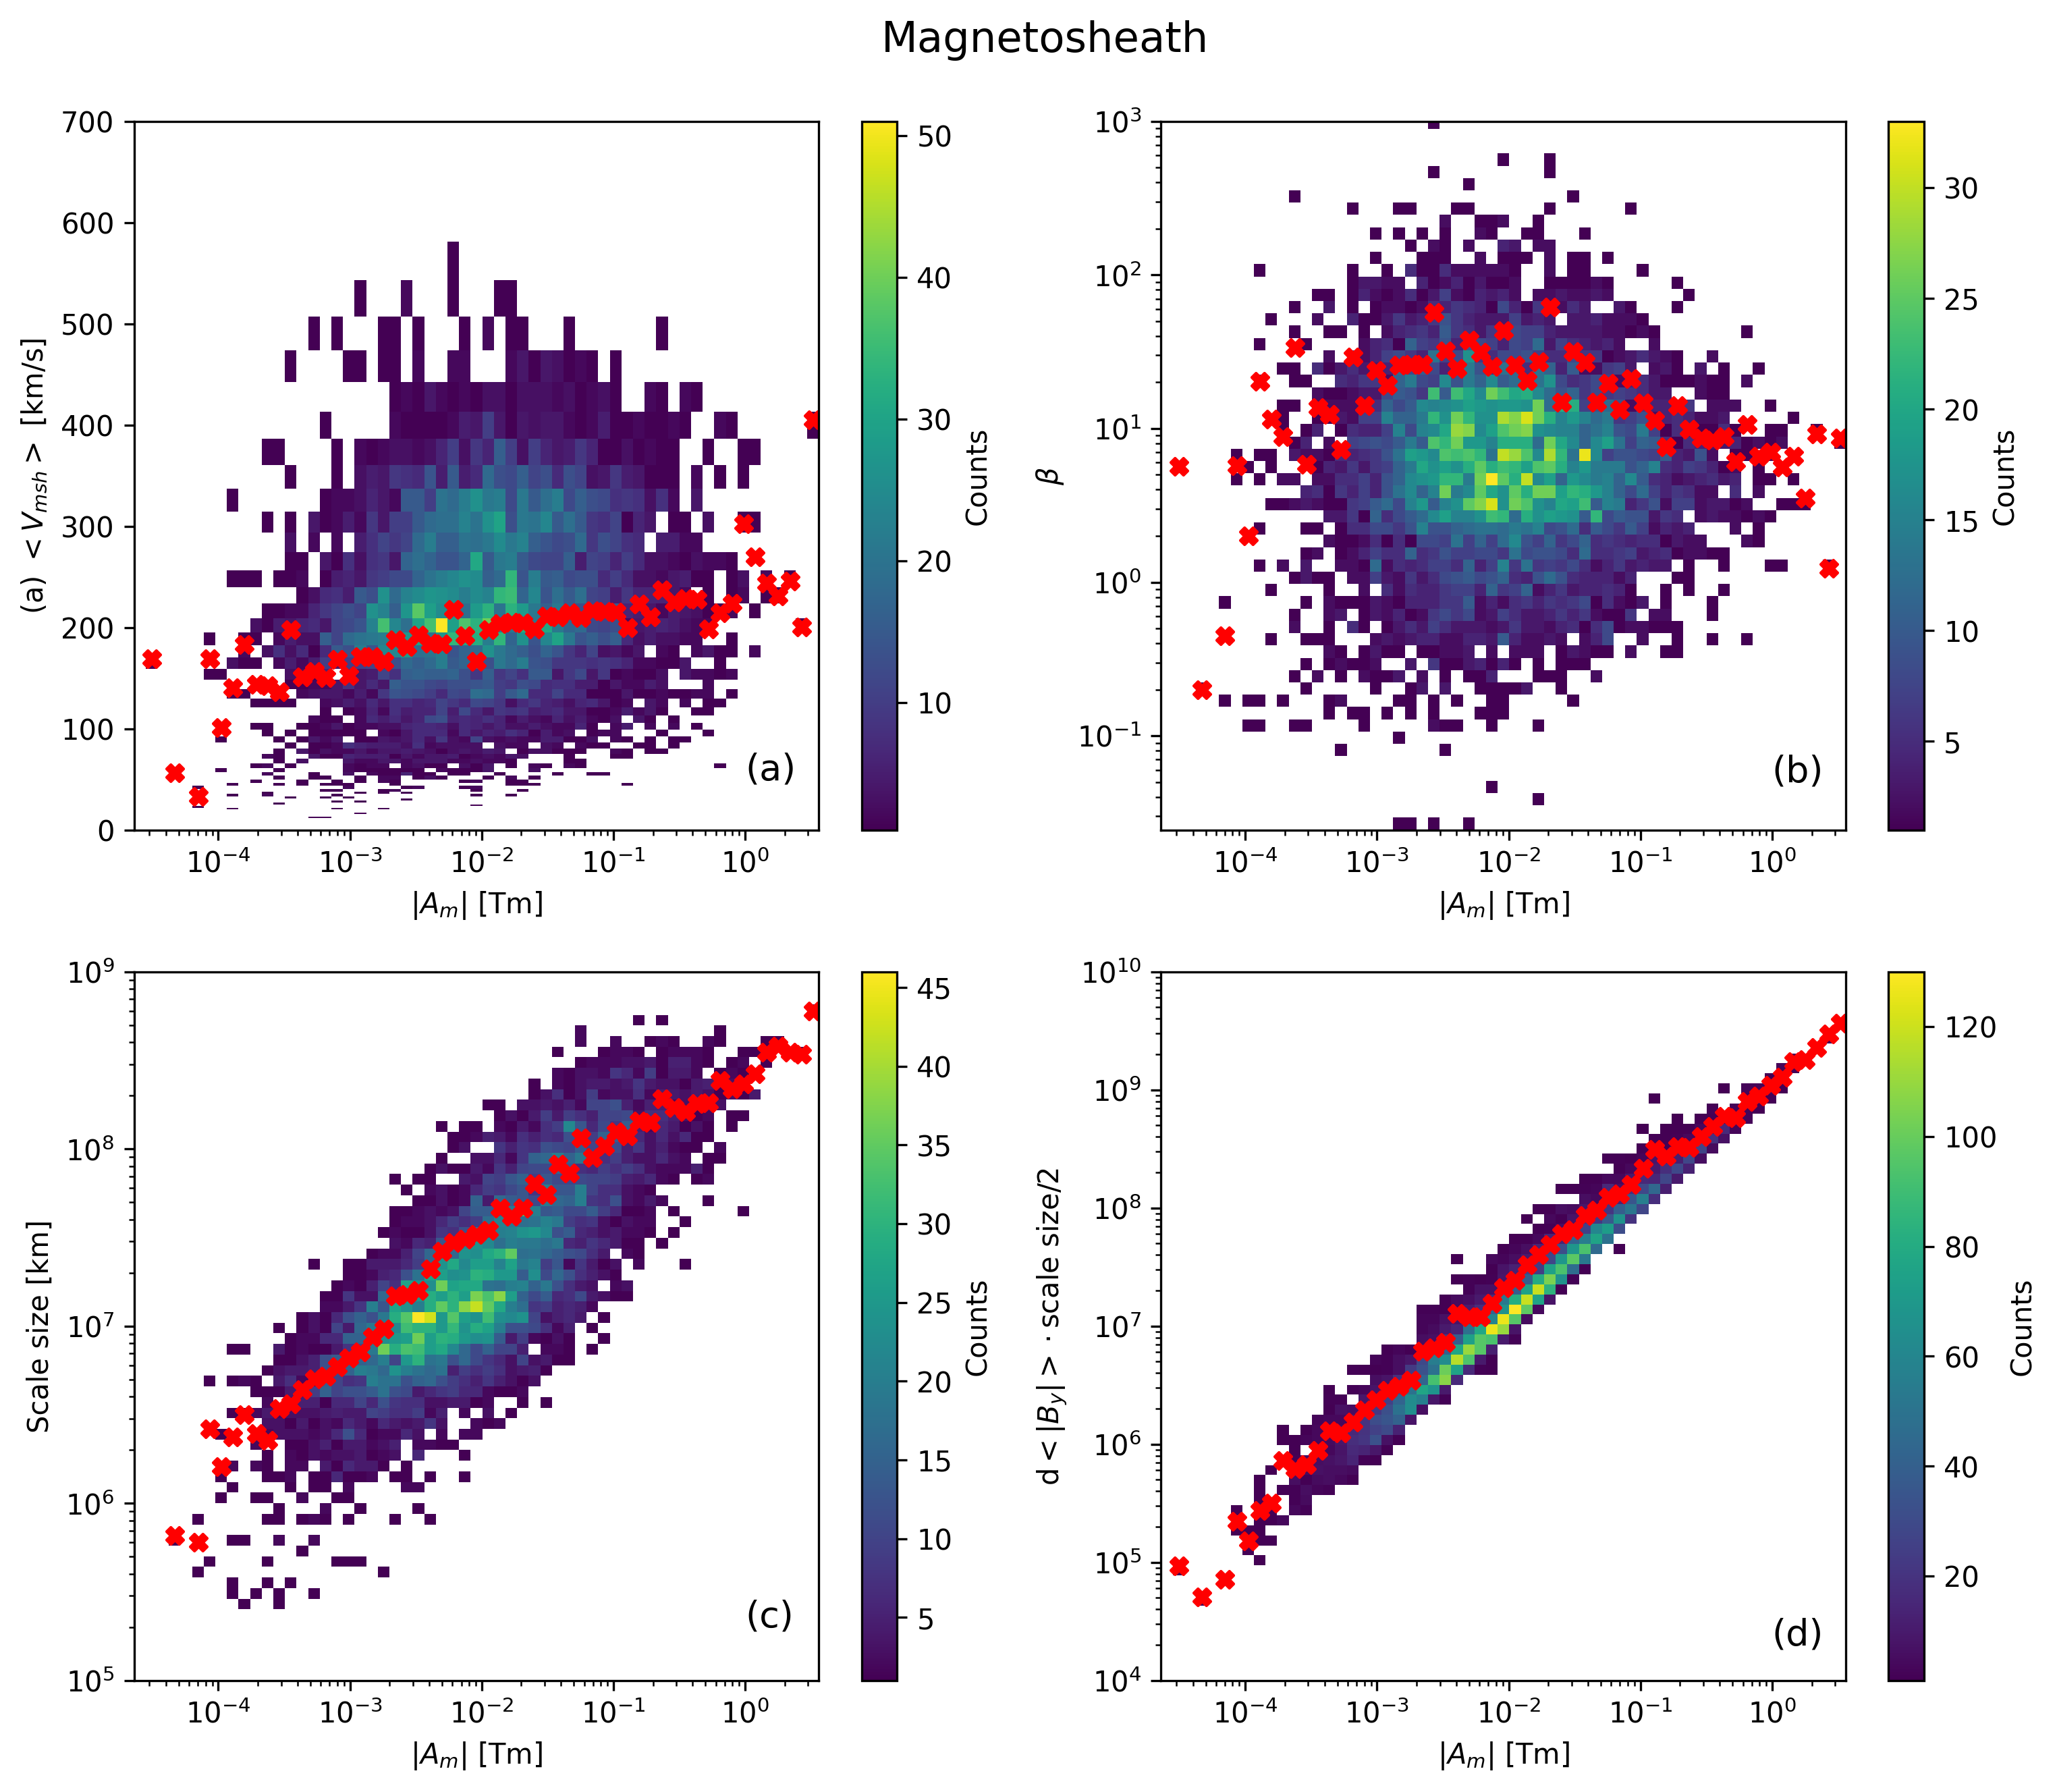
\includegraphics[width=0.45\linewidth]{Figures/GS analysis/heatmap_magnetosheath.png}
    \caption[2D distributions of various parameters vs. $|A_m|$]{Caption}
    \label{fig:heatmap-A}
\end{figure}

\section{Flow velocities and orientation of SFRs}
Lastly, a representation of the average flow velocities of the identified event intervals, i.e., $\mathbf{V_{HT}}$ vectors, is shown in Figure \ref{fig:VHT-xy}. For the identified SFR structures, we find that the corresponding flow velocities in the solar wind are fairly uniform and along the Sun-Earth direction; however, in the magnetosheath the flows appear to be largely deflected toward the duskside flank. Therefore the structures near the flanks (downstream of the quasi-perpendicular portion of the bow shock) ought to have elongated cross sections, resulting in large scale sizes. It is likely that while the structures may be compressed by the bow shock in the dimension along the normal direction of the bow shock, they may experience stretching along the dimension in the direction of the bulk flows, i.e., approximately perpendicular to the normal direction. This explains why some structures in the magnetosheath have large scale sizes, for instance, larger than the typical width of the magnetosheath itself.

\begin{figure}
    \centering
    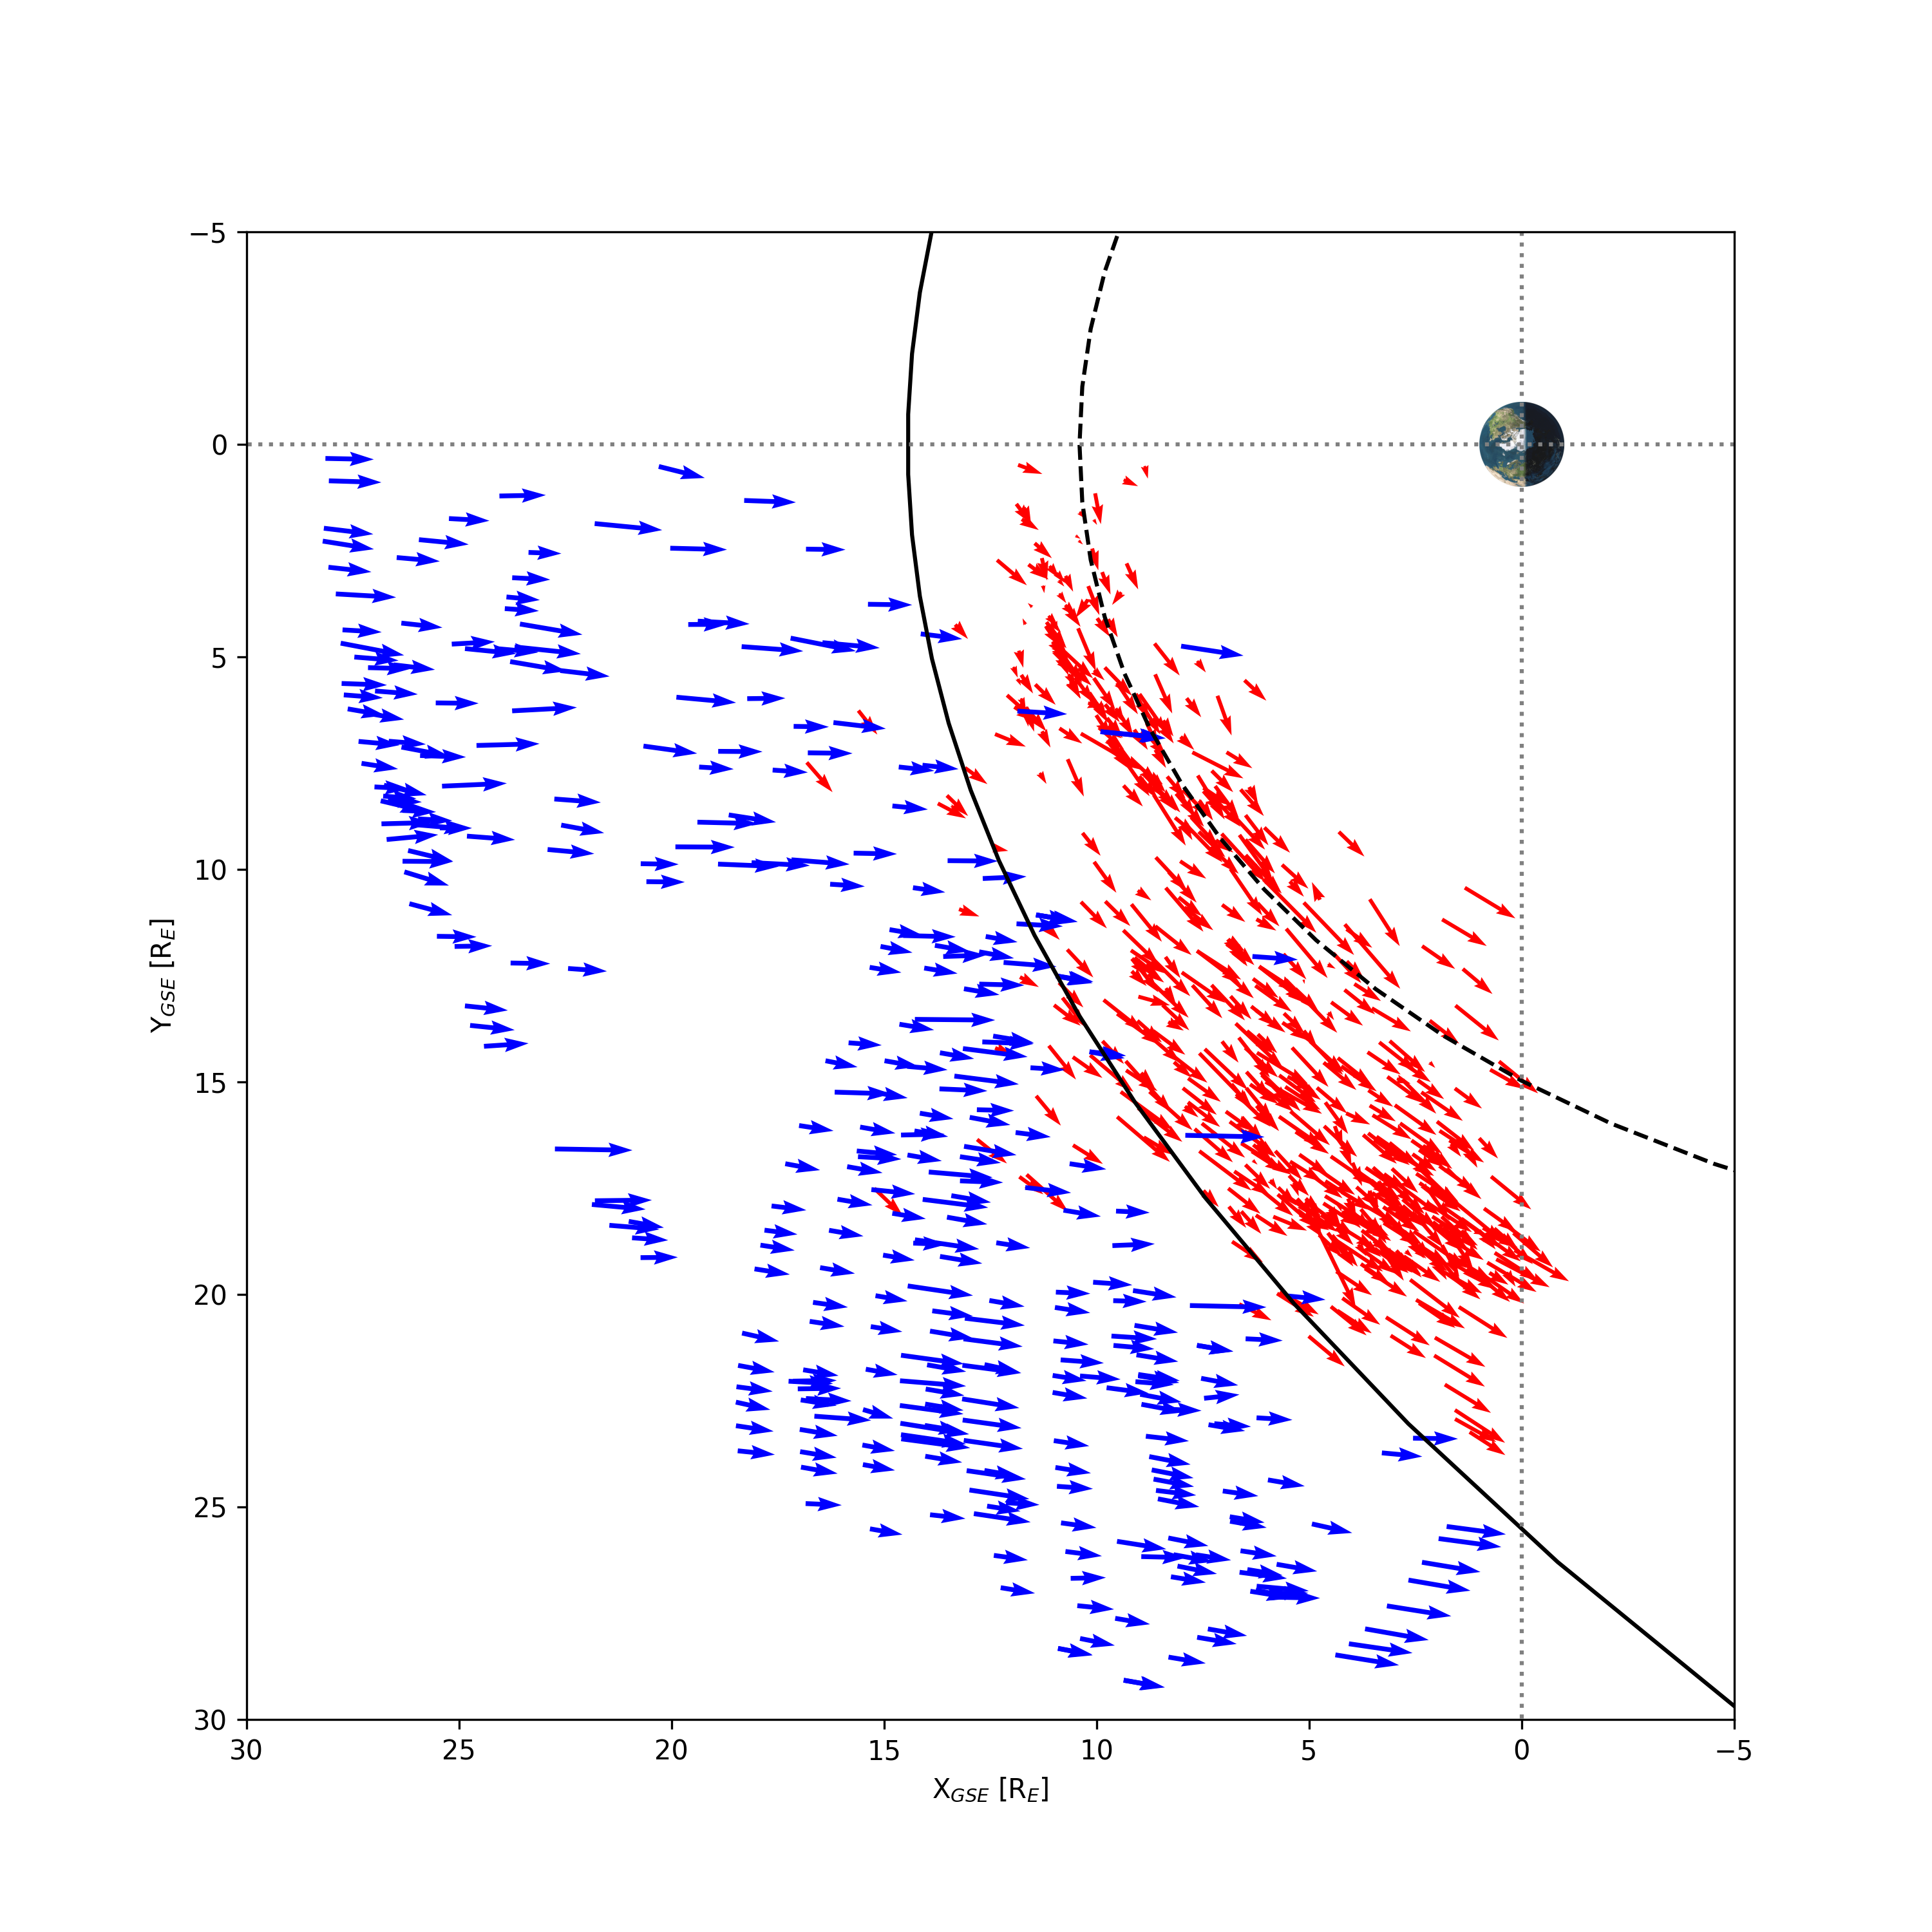
\includegraphics[width=\textwidth]{Figures/Orbits/VHT_xy.png}
    \caption[Orbit plot of flow vectors associated with the SFRs]{Plot showing the $\mathbf{V_{HT}}$ vectors at the locations of one-tenth of the total events identified in the solar wind (blue) and magnetosheath (red) on the GSE-$XY$ plane. The nominal bow shock (solid curve) and magnetopause (dashed curve) locations are drawn based on the models by \citet{Shue:1997} and \citet{SlavinHolzer:1984}, respectively. A reference vector of magnitude 400 km/s is shown in the upper left corner.}
    \label{fig:VHT-xy}
\end{figure}

\begin{figure}
    \centering
    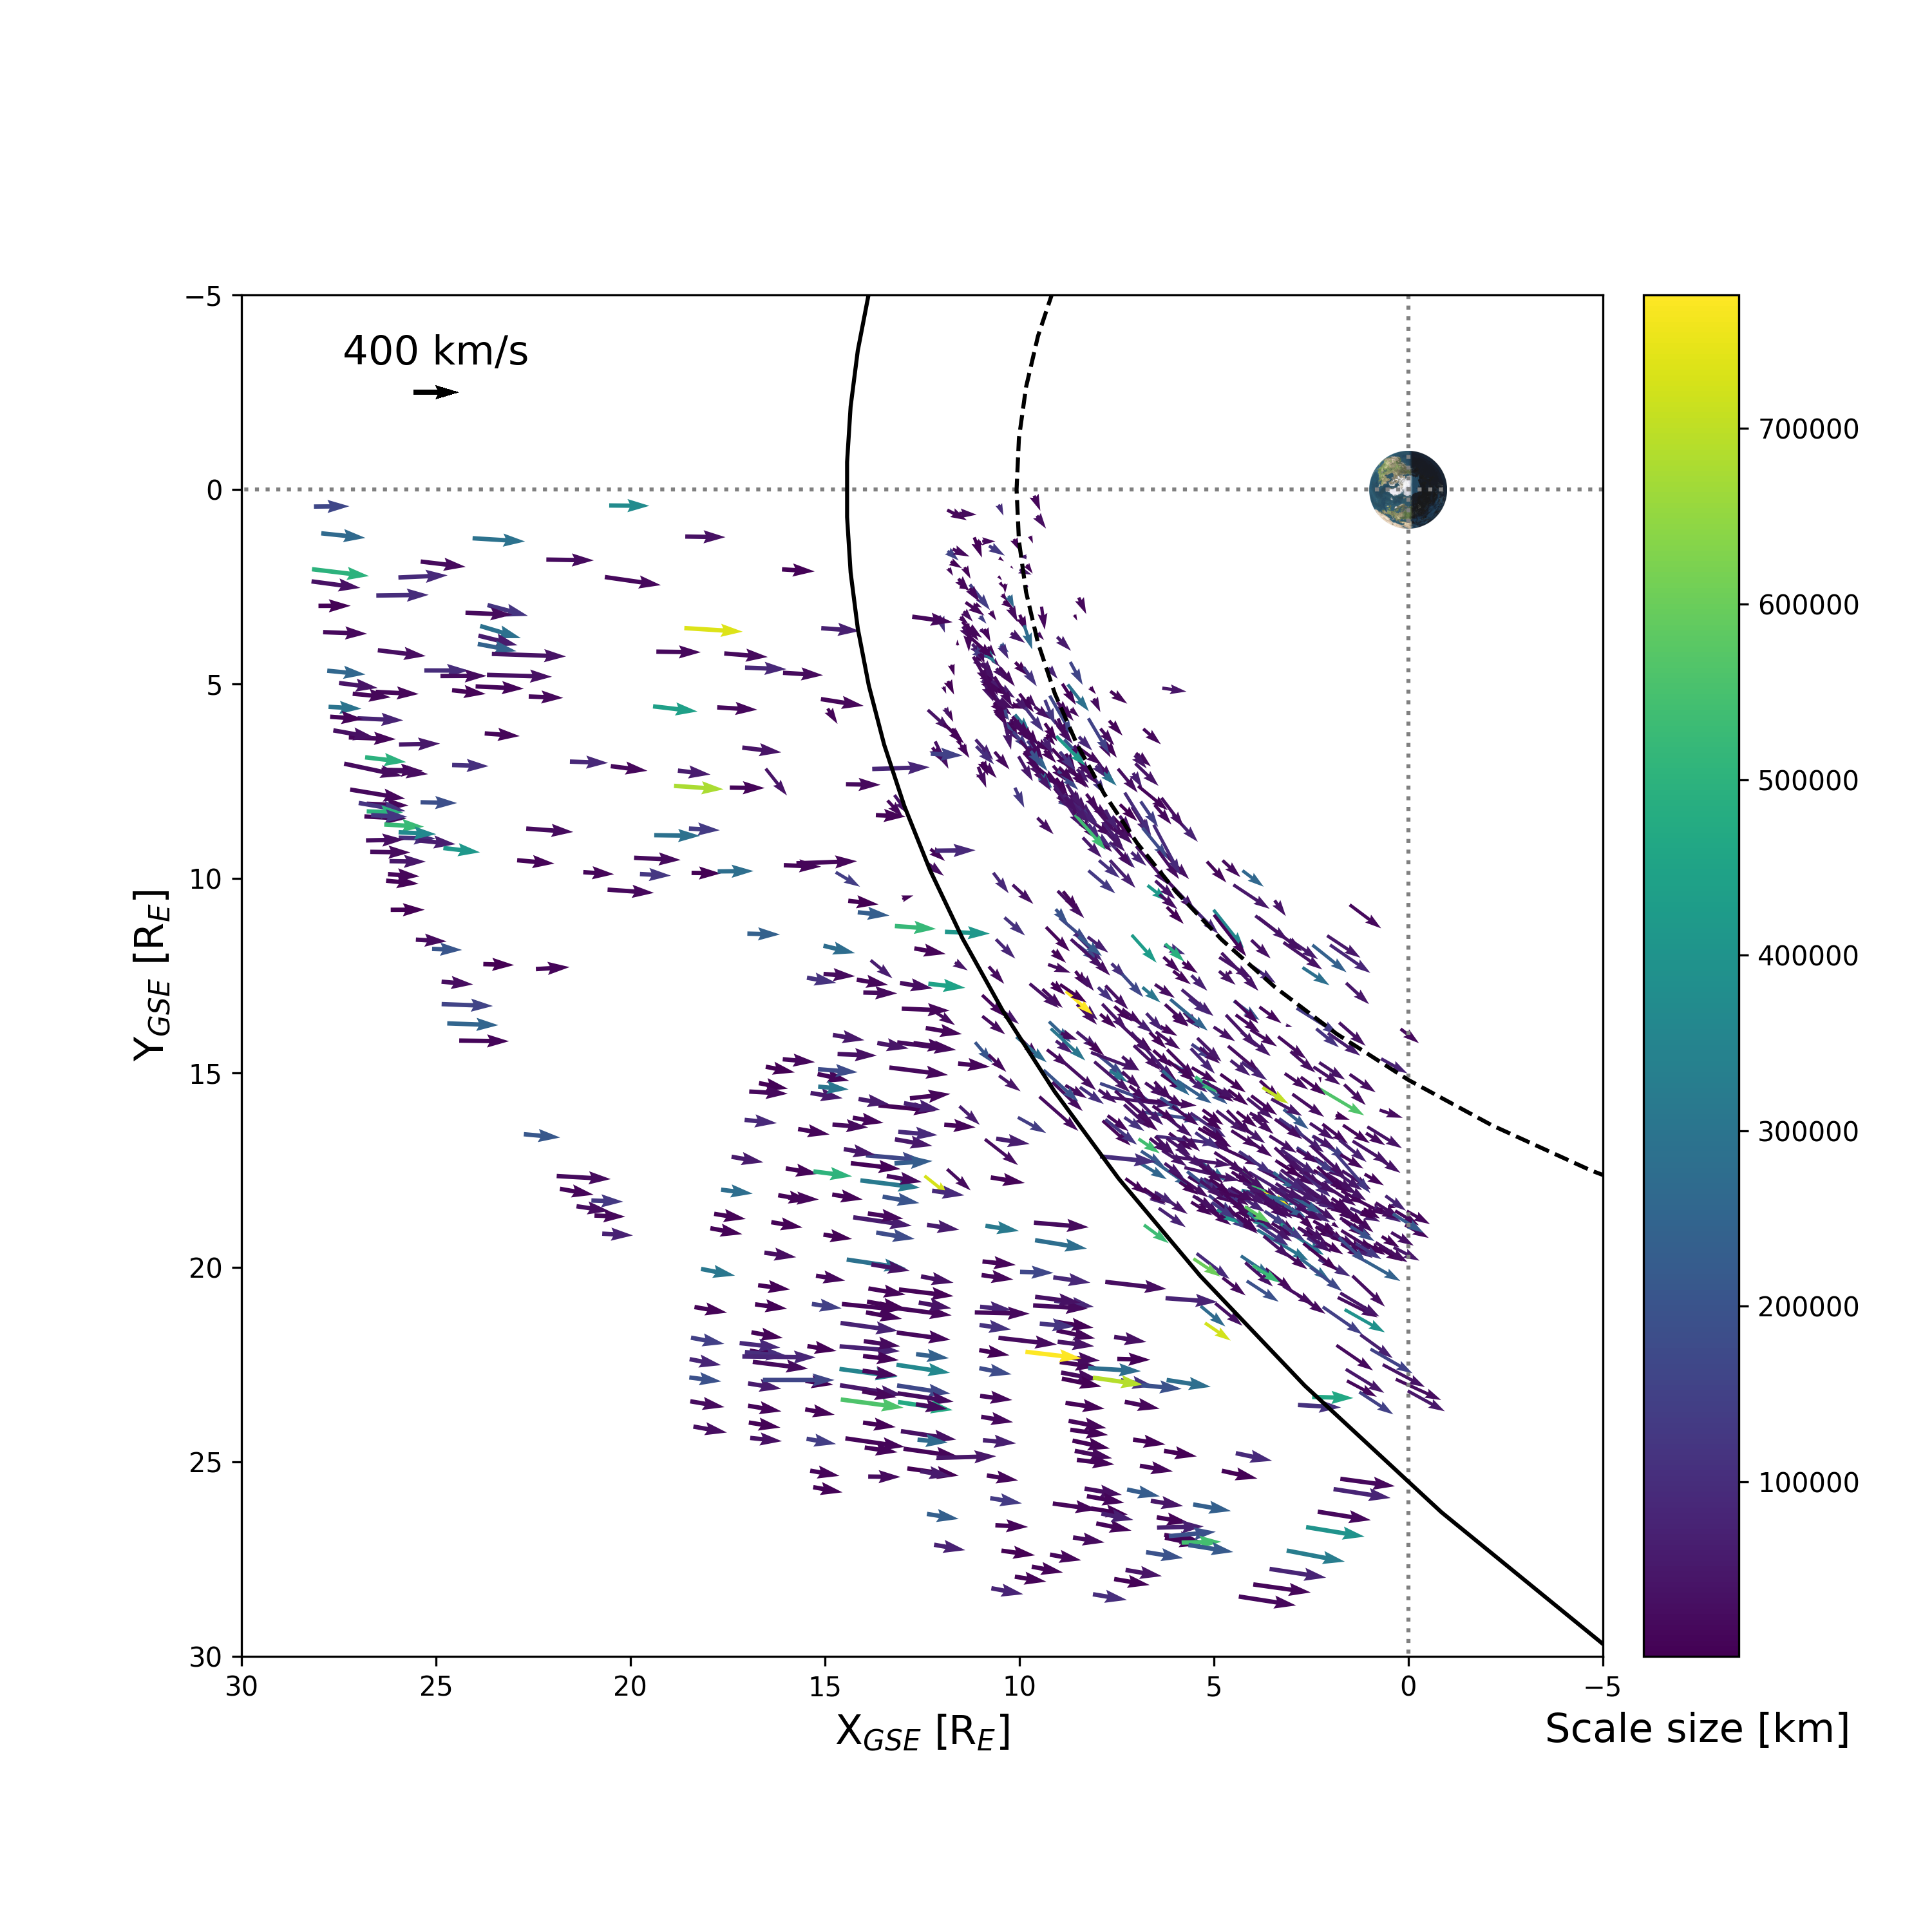
\includegraphics[width=\textwidth]{Figures/Orbits/VHT_xy_scalesize.png}
    \caption[Orbit plot of flow vectors associated with the SFRs, in relation to their scale size]{Plot showing the $\mathbf{V_{HT}}$ vectors at the locations of one-tenth of the total events identified in the solar wind and magnetosheath on the GSE-$XY$ plane. The color gradient indicates the scale size of the SFRs associated with the $\mathbf{V_{HT}}$ vectors. The nominal bow shock (solid curve) and magnetopause (dashed curve) locations are drawn based on the models by \citet{Shue:1997} and \citet{SlavinHolzer:1984}, respectively. A reference vector of magnitude 400 km/s is shown in the upper left corner.}
    \label{fig:VHT-scalesize}
\end{figure}